\documentclass[10pt]{beamer}
\usetheme{Madrid}
\usecolortheme{orchid}
\usepackage[utf8]{inputenc}
\PassOptionsToPackage{hyphens}{url}
\usepackage{hyperref}
\usepackage{graphicx}
\usepackage{booktabs}
\usepackage{array}
\hypersetup{colorlinks=true, urlcolor=blue, linkcolor=black, breaklinks=true}
\urlstyle{same}

\title[Civic Services Monitoring]{Civic Services Surveillance \& Monitoring}
\subtitle{On-device YOLO11n detection of 7 civic issues — dataset sources and training pipeline}
\author{}
\institute{}
\date{August 2026}

\begin{document}

% ---------------------------------------------------------------
\begin{frame}
  \titlepage
\end{frame}

% ---------------------------------------------------------------
\begin{frame}{Agenda}
  \tableofcontents
\end{frame}

\section{Problem Statement}
% ---------------------------------------------------------------
\begin{frame}{Problem Statement}
  \textbf{Civic Services Surveillance \& Monitoring} — real-time, on-device detection of 7 civic issues:
  \begin{enumerate}
    \item Garbage on road ($>$1m accumulations)
    \item Road potholes ($>$10 inch)
    \item Open / broken manholes
    \item Non-working streetlights
    \item Encroachments (unauthorized occupation/obstruction)
    \item Billboard \& hoarding compliance
    \item Cattle on road
  \end{enumerate}
  Each detection auto-generates an incident report: image, camera details, timestamp.
\end{frame}

\section{Approach}
% ---------------------------------------------------------------
\begin{frame}{Approach \& Architecture}
  \begin{itemize}
    \item \textbf{Single unified detector}, not 7 separate models — one YOLO11n running all 7
      classes simultaneously is far cheaper on a phone than 7 models.
    \item \textbf{Model}: YOLO11n (Ultralytics) — chosen over YOLOv8n/YOLOv10n/YOLO-NAS/
      MobileNet-SSD/EfficientDet-Lite/NanoDet for the best size/speed/mobile-export tradeoff.
      $\sim$5--6MB, one-command export to TFLite/ONNX/CoreML.
    \item \textbf{Deployment}: native Android app (CameraX + TFLite), fully offline —
      no internet required for detection.
    \item \textbf{Streetlight state}: no dataset anywhere labels lit/unlit streetlights, so
      the model only localizes the pole; a brightness heuristic classifies lit/unlit at night.
    \item \textbf{Reporting}: every confirmed detection saves a cropped image + JSON
      (class, confidence, timestamp, camera ID) automatically.
  \end{itemize}
\end{frame}

% ---------------------------------------------------------------
\begin{frame}{Dataset Pipeline Overview}
  \begin{itemize}
    \item Datasets sourced from \textbf{Roboflow Universe}, filtered/remapped per class
      into one unified YOLO-format dataset.
    \item \textbf{16,766 images} total, split \textbf{80.1\% train / 19.9\% val}
      (13,435 / 3,331 images).
    \item Split ratio inherited from each source's own train/valid partition — not a custom
      stratified split.
    \item No independently held-out test set beyond the val split used for monitoring.
  \end{itemize}
  \begin{table}
    \centering\small
    \begin{tabular}{lrr}
      \toprule
      Class & Images & \% of dataset \\
      \midrule
      garbage\_pile        & 6{,}350 & 37.9\% \\
      pothole              & 3{,}753 & 22.4\% \\
      billboard\_hoarding  & 3{,}399 & 20.3\% \\
      streetlight\_pole    & 1{,}232 & 7.3\%  \\
      manhole\_open\_broken& 964     & 5.8\%  \\
      encroachment         & 621     & 3.7\%  \\
      cattle               & 447     & 2.7\%  \\
      \bottomrule
    \end{tabular}
  \end{table}
\end{frame}

\section{Datasets by Class}

% ---------------------------------------------------------------
\begin{frame}{garbage\_pile — 6{,}350 images}
  \begin{columns}[T]
    \begin{column}{0.48\textwidth}
      \textbf{Sources:}
      \begin{itemize}
        \small
        \item \textbf{TACO} — 3{,}572 img \\
          \url{https://universe.roboflow.com/mohamed-traore-2ekkp/taco-trash-annotations-in-context} \\
          Non-India (international litter photos)
        \item \textbf{Trash Detection (Roboflow)} — 2{,}778 img \\
          \url{https://universe.roboflow.com/yolo-hfplh/trash-detection-1fjjc-nd1dg} \\
          Origin unconfirmed
      \end{itemize}
    \end{column}
    \begin{column}{0.5\textwidth}
      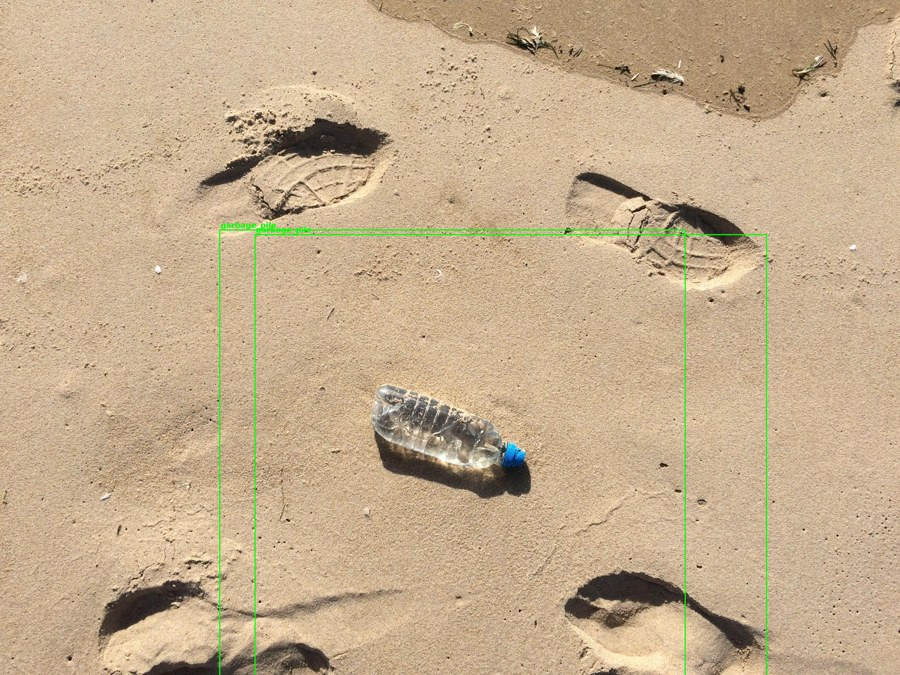
\includegraphics[width=0.95\textwidth]{images/garbage_pile_1.jpg}\\[2pt]
      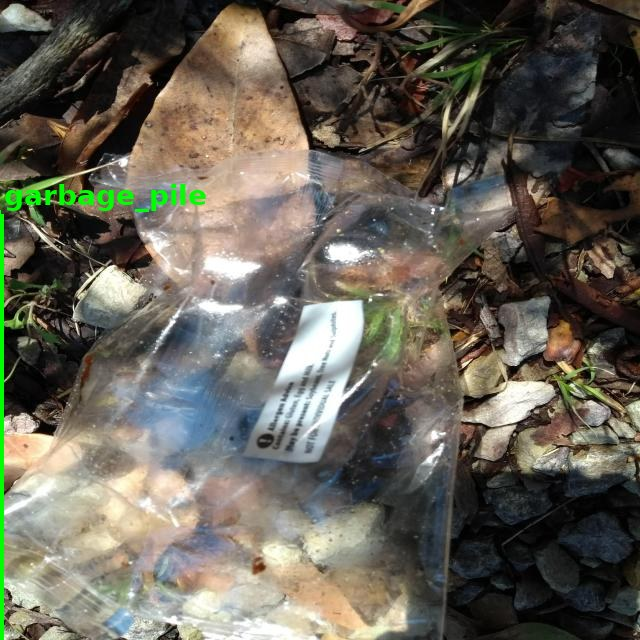
\includegraphics[width=0.47\textwidth]{images/garbage_pile_2.jpg}
      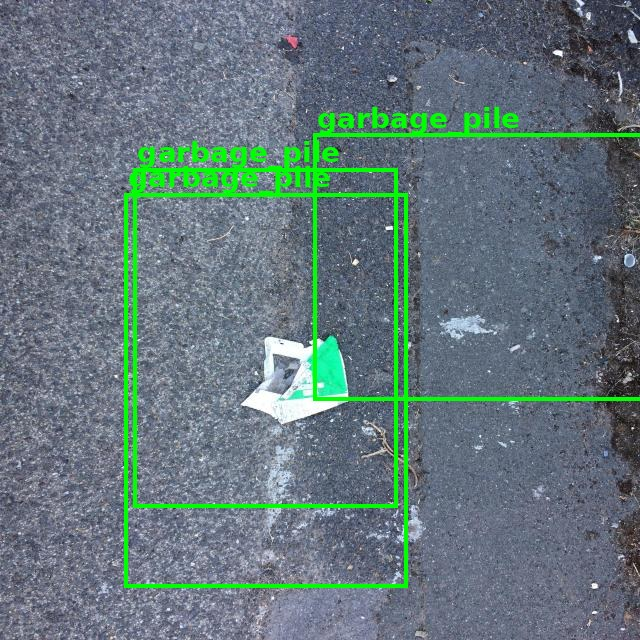
\includegraphics[width=0.47\textwidth]{images/garbage_pile_3.jpg}
    \end{column}
  \end{columns}
\end{frame}

% ---------------------------------------------------------------
\begin{frame}{pothole — 3{,}753 images}
  \begin{columns}[T]
    \begin{column}{0.48\textwidth}
      \textbf{Source:}
      \begin{itemize}
        \small
        \item \textbf{Pothole Detection — Intel Unnati Training Program} — 3{,}753 img \\
          \url{https://universe.roboflow.com/intel-unnati-training-program/pothole-detection-bqu6s} \\
          \textbf{India} (Intel Unnati is an India-based program)
      \end{itemize}
      \vspace{6pt}
      Best-performing detection-only class besides cattle — AP50 0.85.
    \end{column}
    \begin{column}{0.5\textwidth}
      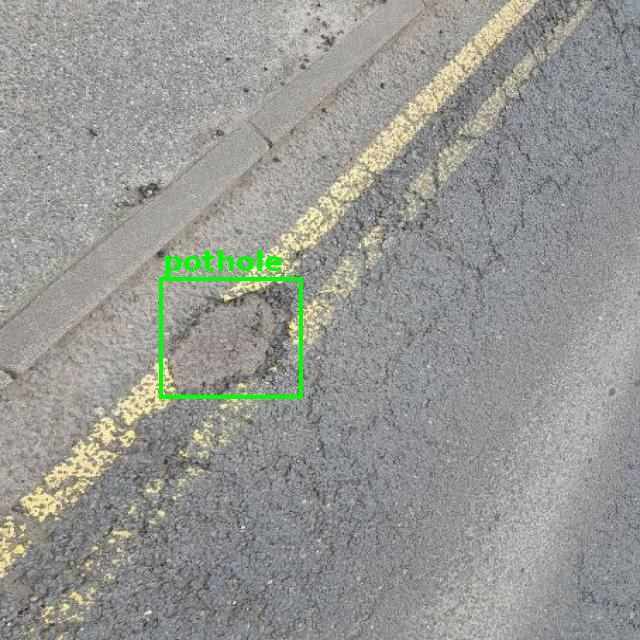
\includegraphics[width=0.95\textwidth]{images/pothole_1.jpg}\\[2pt]
      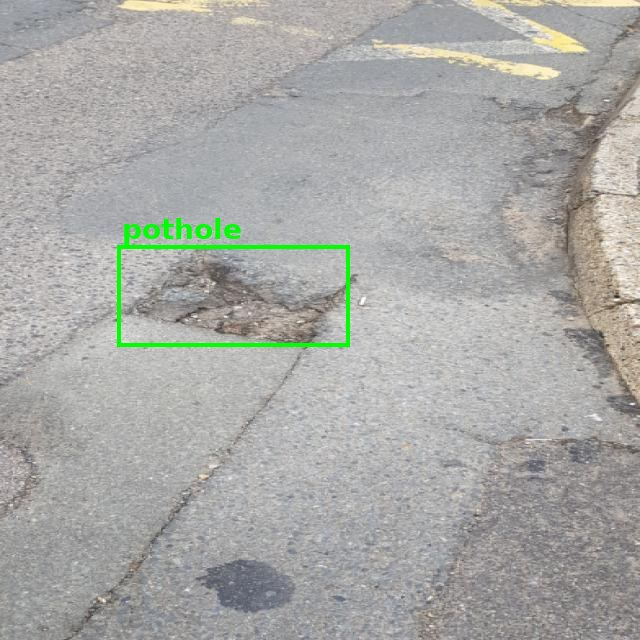
\includegraphics[width=0.47\textwidth]{images/pothole_2.jpg}
      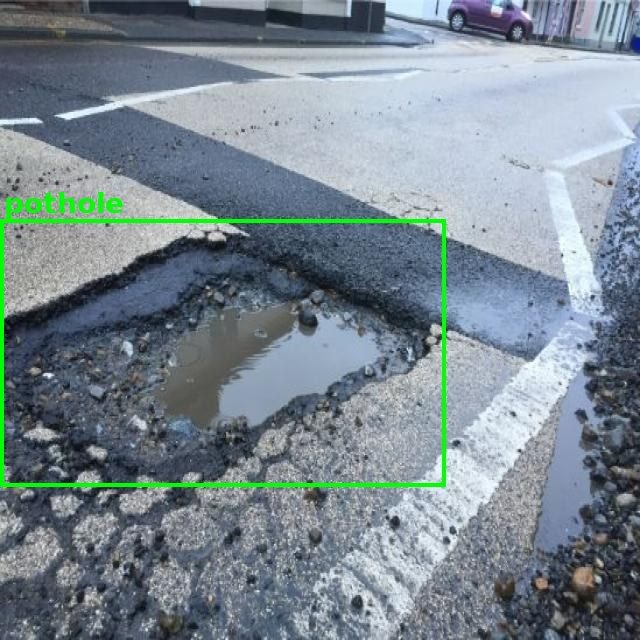
\includegraphics[width=0.47\textwidth]{images/pothole_3.jpg}
    \end{column}
  \end{columns}
\end{frame}

% ---------------------------------------------------------------
\begin{frame}{manhole\_open\_broken — 964 images}
  \begin{columns}[T]
    \begin{column}{0.48\textwidth}
      \textbf{Sources} (filtered to broken/open/uncovered classes only):
      \begin{itemize}
        \small
        \item \textbf{Manhole Cover Dataset YOLO} — 467 img \\
          \url{https://universe.roboflow.com/create-dataset-for-yolo/manhole-cover-dataset-yolo}
        \item \textbf{Open-Manholes} — 444 img \\
          {\scriptsize\url{https://universe.roboflow.com/aibased-solution-for-realtime-detection-of-road-anomalies-d6eay/open-manholes}}
        \item \textbf{Manhole Broken v2} — 53 img \\
          \url{https://universe.roboflow.com/2nd-workspace/manhole-broken}
        \item All origins unconfirmed
      \end{itemize}
    \end{column}
    \begin{column}{0.5\textwidth}
      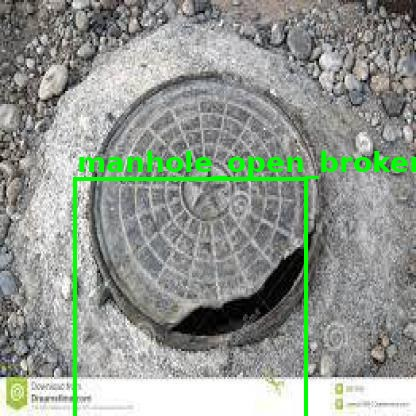
\includegraphics[width=0.95\textwidth]{images/manhole_open_broken_1.jpg}\\[2pt]
      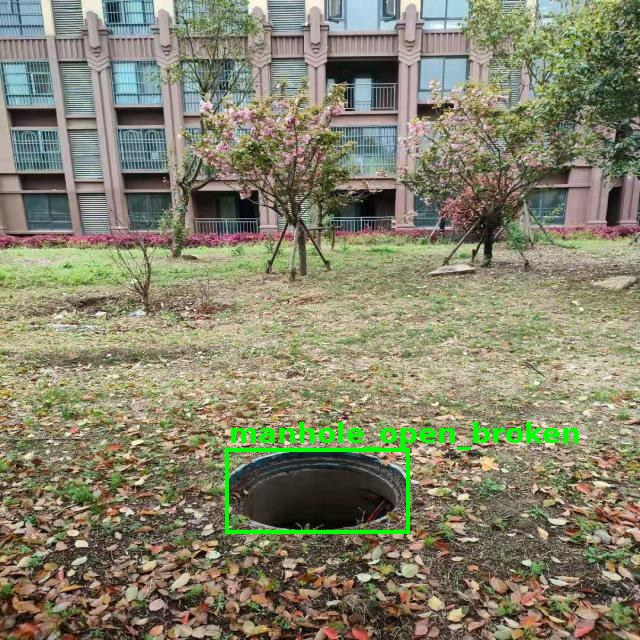
\includegraphics[width=0.47\textwidth]{images/manhole_open_broken_2.jpg}
      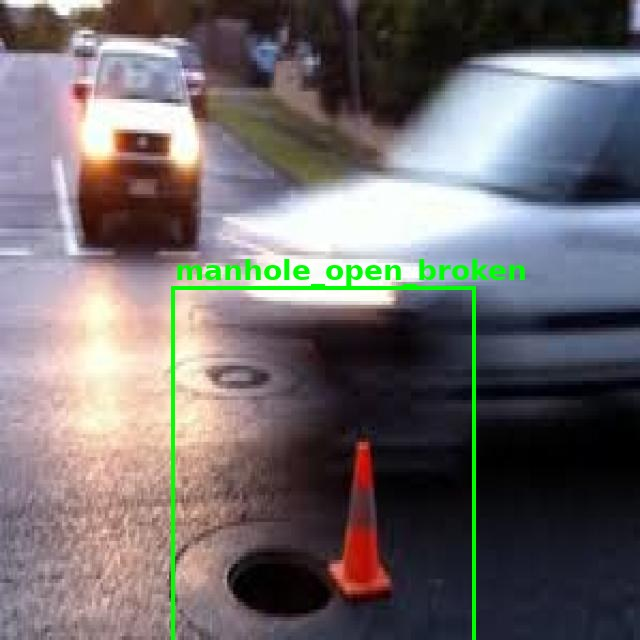
\includegraphics[width=0.47\textwidth]{images/manhole_open_broken_3.jpg}
    \end{column}
  \end{columns}
\end{frame}

% ---------------------------------------------------------------
\begin{frame}{streetlight\_pole — 1{,}232 images}
  \begin{columns}[T]
    \begin{column}{0.48\textwidth}
      \textbf{Source:}
      \begin{itemize}
        \small
        \item \textbf{Street Light (Sashank S)} — 1{,}232 img \\
          \url{https://universe.roboflow.com/sashank-s/street-light} \\
          Origin unconfirmed
      \end{itemize}
      \vspace{6pt}
      \textbf{Note:} localizes the pole only — no dataset anywhere labels
      lit/unlit state. On/off is inferred at inference time via a brightness
      heuristic on the cropped region at night, not a learned label.
    \end{column}
    \begin{column}{0.5\textwidth}
      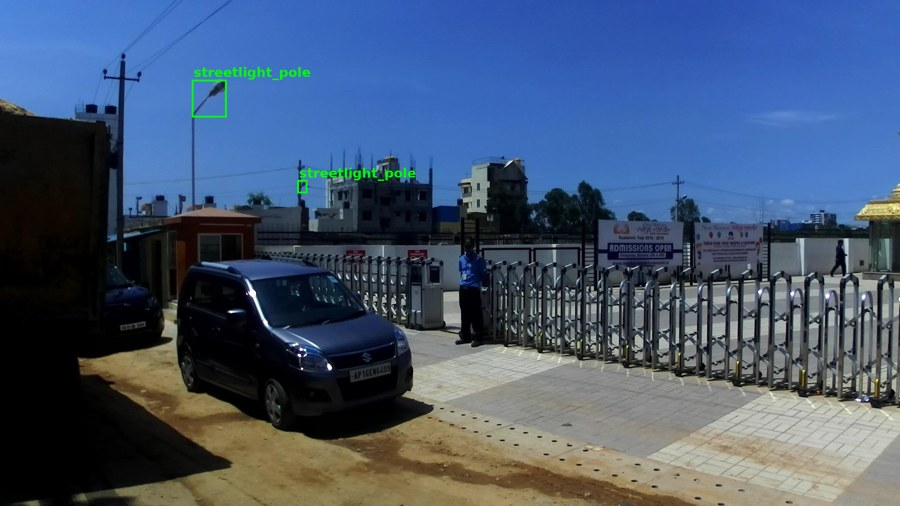
\includegraphics[width=0.95\textwidth]{images/streetlight_pole_1.jpg}\\[2pt]
      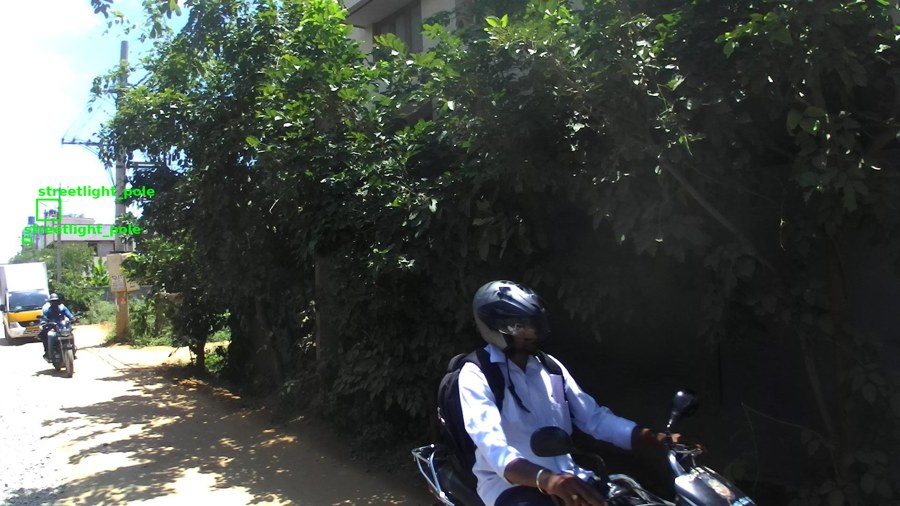
\includegraphics[width=0.47\textwidth]{images/streetlight_pole_2.jpg}
      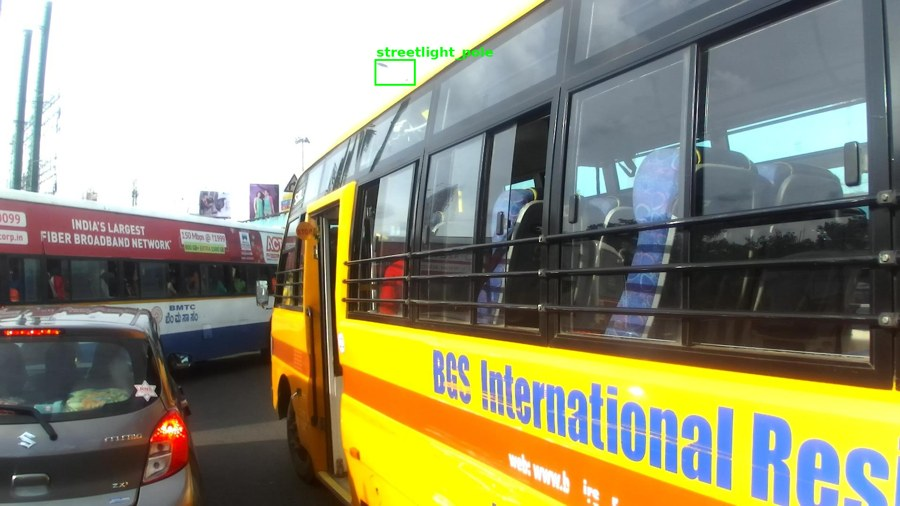
\includegraphics[width=0.47\textwidth]{images/streetlight_pole_3.jpg}
    \end{column}
  \end{columns}
\end{frame}

% ---------------------------------------------------------------
\begin{frame}{encroachment — 621 images}
  \begin{columns}[T]
    \begin{column}{0.48\textwidth}
      \textbf{Sources:}
      \begin{itemize}
        \small
        \item \textbf{Street Vendors (public)} — 495 img \\
          \url{https://universe.roboflow.com/public-2mrlb/street-vendors}
        \item \textbf{Street Vendors India} — 59 img \\
          \url{https://universe.roboflow.com/mit-f83x1/street-vendors-india} \\
          \textbf{India}
        \item \textbf{Footpath Guide} (filtered to Vendor/Vendor cart/\newline Obstacle/Street goods) — 65 img \\
          \url{https://universe.roboflow.com/vendor/footpath-guide}
        \item Illegal Parking (original) — 2 img
      \end{itemize}
      \vspace{4pt}
      \small\textbf{Weakest class}: started with only 2 usable images (AP50 0.00);
      after adding these sources, AP50 improved to 0.35.
    \end{column}
    \begin{column}{0.5\textwidth}
      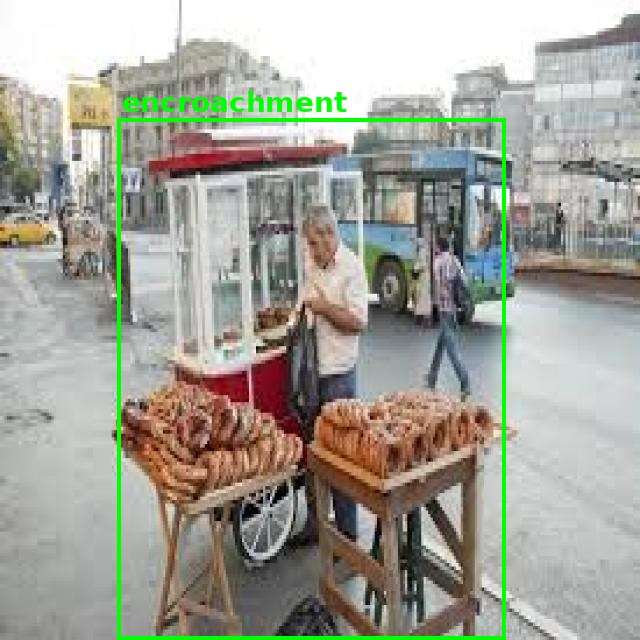
\includegraphics[width=0.95\textwidth]{images/encroachment_1.jpg}\\[2pt]
      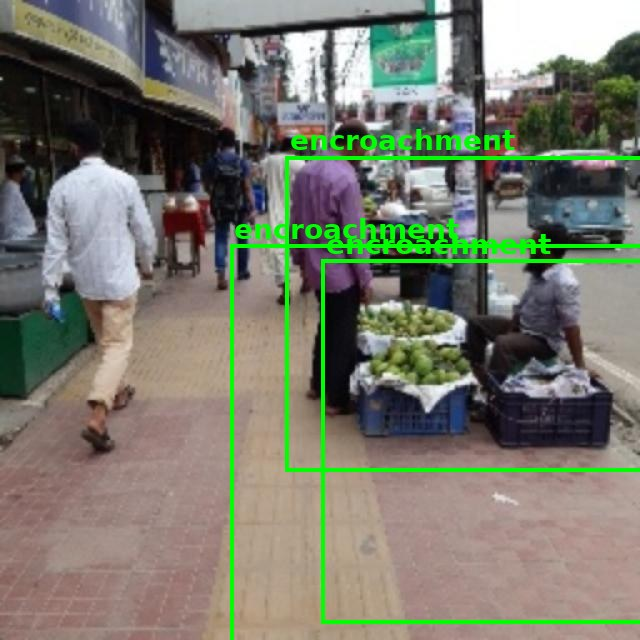
\includegraphics[width=0.47\textwidth]{images/encroachment_2.jpg}
      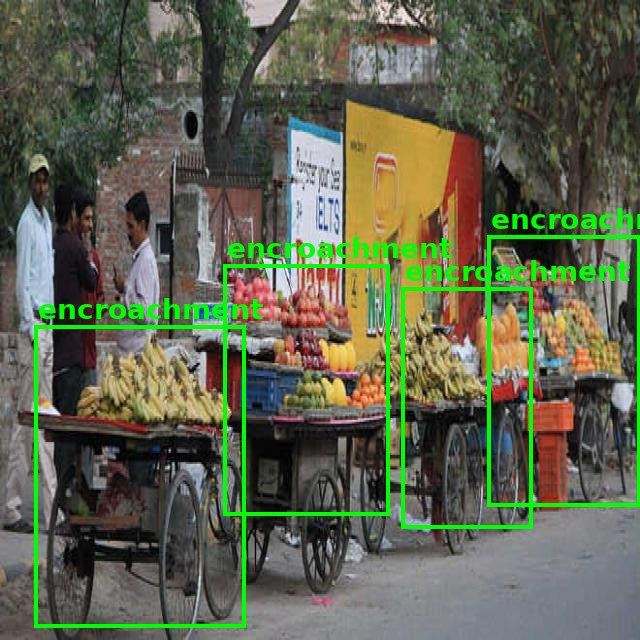
\includegraphics[width=0.47\textwidth]{images/encroachment_3.jpg}
    \end{column}
  \end{columns}
\end{frame}

% ---------------------------------------------------------------
\begin{frame}{billboard\_hoarding — 3{,}399 images}
  \begin{columns}[T]
    \begin{column}{0.48\textwidth}
      \textbf{Source:}
      \begin{itemize}
        \small
        \item \textbf{Billboard Object Detection (Roboflow)} — 3{,}399 img \\
          \url{https://universe.roboflow.com/arslan-ongr8/billboard-xlvz1} \\
          Origin unconfirmed
      \end{itemize}
      \vspace{6pt}
      \textbf{Note:} detects billboard/hoarding presence only — no dataset provides
      ground-truth permit or size-compliance labels, so ``compliance'' checking is
      not implemented, only localization.
    \end{column}
    \begin{column}{0.5\textwidth}
      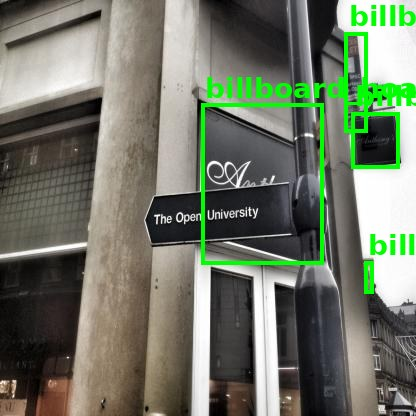
\includegraphics[width=0.95\textwidth]{images/billboard_hoarding_1.jpg}\\[2pt]
      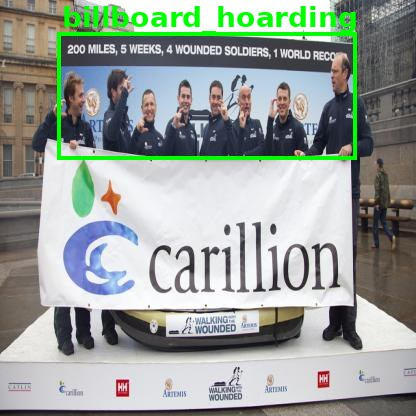
\includegraphics[width=0.47\textwidth]{images/billboard_hoarding_2.jpg}
      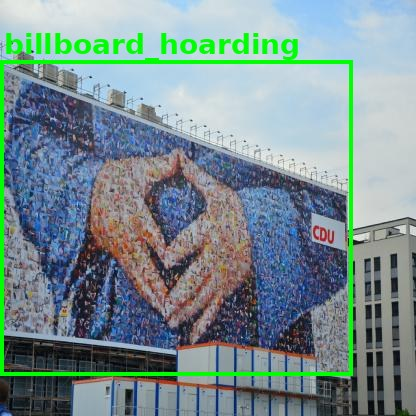
\includegraphics[width=0.47\textwidth]{images/billboard_hoarding_3.jpg}
    \end{column}
  \end{columns}
\end{frame}

% ---------------------------------------------------------------
\begin{frame}{cattle — 447 images}
  \begin{columns}[T]
    \begin{column}{0.48\textwidth}
      \textbf{Source:}
      \begin{itemize}
        \small
        \item \textbf{Cow Indian (Roboflow)} — 447 img \\
          \url{https://universe.roboflow.com/sakshi-kumari-70uxi/cow-indian} \\
          \textbf{India} (explicitly ``stray cattle on Indian roads'')
      \end{itemize}
      \vspace{6pt}
      Best-performing class overall — AP50 0.99. COCO/Open-Images pretrained
      weights already include a \texttt{cow} class, giving this class a head start.
    \end{column}
    \begin{column}{0.5\textwidth}
      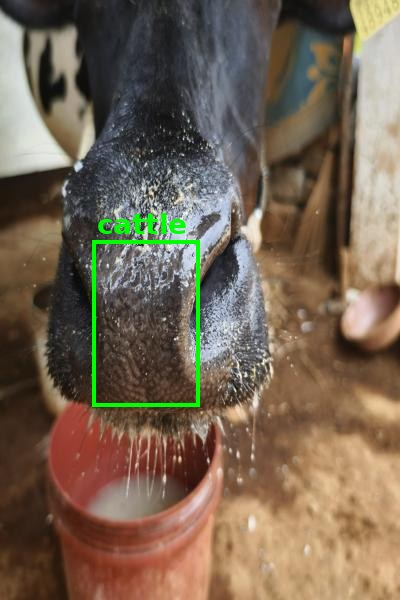
\includegraphics[width=0.95\textwidth]{images/cattle_1.jpg}\\[2pt]
      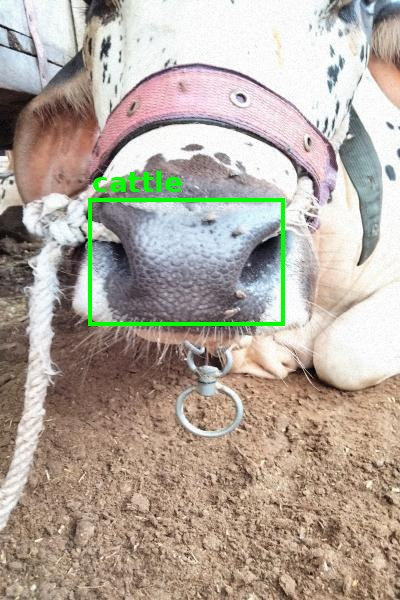
\includegraphics[width=0.47\textwidth]{images/cattle_2.jpg}
      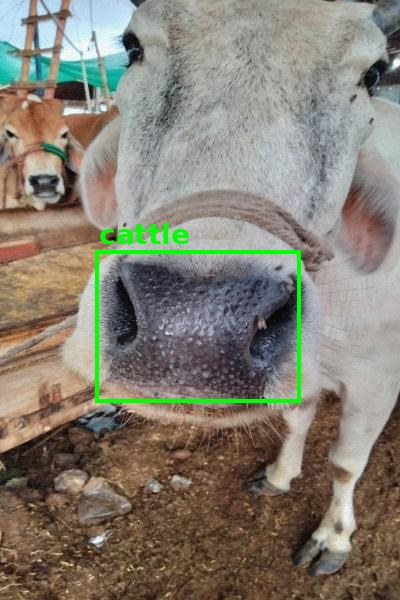
\includegraphics[width=0.47\textwidth]{images/cattle_3.jpg}
    \end{column}
  \end{columns}
\end{frame}

\section{Training Results}
% ---------------------------------------------------------------
\begin{frame}{Training Results — Run 1 vs.\ Run 2 (after adding encroachment data)}
  \begin{table}
    \centering\small
    \begin{tabular}{lrr}
      \toprule
      Class & Run 1 AP50 (16{,}094 img) & Run 2 AP50 (16{,}766 img) \\
      \midrule
      cattle               & 0.992 & 0.986 \\
      pothole              & 0.849 & 0.851 \\
      manhole\_open\_broken& 0.823 & \textbf{0.843} \\
      billboard\_hoarding  & 0.689 & 0.684 \\
      streetlight\_pole    & 0.650 & \textbf{0.661} \\
      garbage\_pile        & 0.608 & \textbf{0.643} \\
      encroachment         & 0.000 & \textbf{0.350} \\
      \midrule
      \textbf{Overall mAP50} & \textbf{0.659} & \textbf{0.717} \\
      Overall mAP50-95     & 0.420 & 0.472 \\
      \bottomrule
    \end{tabular}
  \end{table}
  Both runs: YOLO11n, 100 epochs. Adding encroachment data fixed that class
  entirely without hurting any other class.
\end{frame}

\section{Dataset Origin}
% ---------------------------------------------------------------
\begin{frame}{Dataset Origin — India vs.\ Non-India}
  \begin{table}
    \centering\small
    \begin{tabular}{lr}
      \toprule
       & Images (\% of 16{,}766) \\
      \midrule
      Confirmed India       & 4{,}259 \ (25.4\%) \\
      Confirmed Non-India   & 3{,}572 \ (21.3\%) \\
      Unconfirmed origin    & 8{,}935 \ (53.3\%) \\
      \bottomrule
    \end{tabular}
  \end{table}
  \begin{itemize}
    \item Only 3 of 15 source datasets are confirmed Indian: Intel Unnati (pothole),
      Street Vendors India (encroachment), Cow Indian (cattle).
    \item Most Roboflow community uploads never state geographic origin.
    \item Classes with confirmed Indian data (pothole, cattle) are also the
      best-performing — plausible but unproven relationship.
    \item Real-world accuracy on Indian roads for garbage/manhole/streetlight/billboard
      may be lower than validation numbers suggest.
  \end{itemize}
\end{frame}

\section{Android App}
% ---------------------------------------------------------------
\begin{frame}{Android App}
  \begin{itemize}
    \item Native app: CameraX + TFLite, fully on-device, works with \textbf{no internet}.
    \item Live detection overlay with FPS/detection counter.
    \item Manual photo capture and video recording alongside live detection.
    \item Automatic incident reporting: cropped image + JSON per confirmed detection,
      60s per-class cooldown to avoid duplicate spam.
    \item Landing page, Reports gallery, About screen with light/dark mode toggle.
    \item Verified live on a Samsung Galaxy S24 via adb — camera rotation and
      model input-layout bugs were found and fixed by testing against real
      recorded video, not by code inspection alone.
  \end{itemize}
\end{frame}

\section{Limitations}
% ---------------------------------------------------------------
\begin{frame}{Known Limitations}
  \begin{itemize}
    \item No physical size/dimension measurement — garbage ($>$1m) and pothole
      ($>$10in) thresholds from the problem statement are not verified, only
      generic object detection.
    \item No alerting/notification pipeline — reports save locally to the phone only.
    \item No billboard compliance logic (permits, size rules) — detection only.
    \item Streetlight lit/unlit state is a brightness heuristic, not a trained classifier.
    \item Encroachment (AP50 0.35) is still the weakest class — only 621 training images.
    \item No independently held-out test set beyond the validation split.
  \end{itemize}
\end{frame}

% ---------------------------------------------------------------
\begin{frame}{Thank You}
  \centering
  \Large Questions?
\end{frame}

\end{document}
